\begin{problem}{Нить ДНК}{стандартный ввод}{стандартный вывод}{1 секунда}{256 мегабайт}

Тобул серьезно увлекается биологией, и совсем недавно он узнал, что все живые организмы имеют ДНК~--- молекулу-носитель генетической информации. Она состоит из двух цепей, каждая из которых закручена по \textit{цилиндрической винтовой линии}. 

Оказывается, у каждого живого организма молекула ДНК имеет свои параметры~--- своя длина ($L$), радиус витка нити ДНК ($R$), длина шага витка ($h$).

\begin{center}
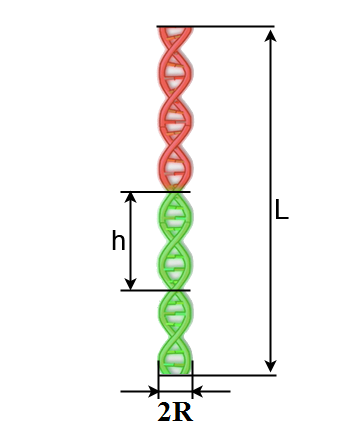
\includegraphics[scale=0.4]{dna.png}
\end{center}

Тобула очень заинтересовал один вопрос: можно ли определить длину нити ДНК для определенного типа живого организма? Поскольку он все свое время посвящает биологии, то с~математикой, к~его большому стыду, у него не очень хорошо. Вот почему он просит вас помочь ему вычислить длину одной нити ДНК живого организма.

\InputFile
На вход вашей программе даются характеристики ДНК живого организма~--- три вещественных числа $L$, $R$, $h$, ($0< L, R, h \le 10^4$). Числа заданы с~точностью до двух знаков после десятичной точки.

\OutputFile
Ваша программа должна вывести длину одной нити ДНК с~точностью до четвертого знака после точки.

\Example

\begin{example}
\exmpfile{example.01}{example.01.a}%
\end{example}

\Note
В ваших вычислениях значение $\pi$ примите равным $3.141593$.

Винтовая линия~--- это пространственная кривая, описываемая точкой $M$, которая вращается с~постоянной угловой скоростью вокруг неподвижной оси $OO^\prime$ и одновременно перемещается вверх с~постоянной скоростью вдоль этой оси.
\begin{center}
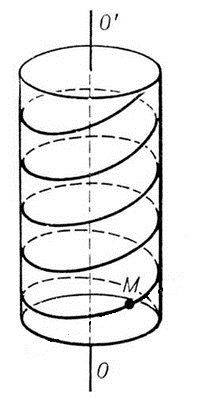
\includegraphics[scale=0.4]{291913915.jpg}
\end{center}

\end{problem}

